\chapter{München}

München er hovedstaden i delstaten Bayern, og har gode 1,3 millioner innbyggere. Hvis en regner med forsteder og grensende landsbyer var det per 2007 2,6 millioner innbyggere. Byen er meget velstående, og har mye industri (elektro, bilindustri, kjemi, media/informatikk og øl). Det er en trygg by å bo i, med lite kriminalitet. 

Byen har noe å by på til enhver sesong. Et flertall av parker, 53 museer (blant annet verdens største tekniske museum: Deutsches Museum), 71 teater, mangfoldige årlige kulturarrangementer og flere konsertscener med et utrolig tilbud. En får ikke glemme de to fotballagene FC Bayern og 1860 München. München er ingen typisk storby, og blir av mange kalt Europas største landsby. Den Engelske Hagen er den største parken, og strekker seg mangfoldige kilometer fra byens sentrum nordover. Her sitter det folk og koser seg med piknik og øl, mens andre spiller fotball eller jogger. Sommersesongen avsluttes med Oktoberfest; verdens største øl-festival.
München ligger ca 580 moh, og de nærliggende alpene når man med en times biltur (Tyske alpene; Zugspitze, Lenggries, Spitzingsee). Kjører man en time til er man i Østerrike, hvor man har et ufattelig utvalg av områder til rådighet. Om sommeren er dette fantastiske turområder, og om vinteren fantastiske skiområder.


Byen ligger også meget sentralt til i forhold til Tsjekkia, Sveits, Italia, Ungarn og Østerrike. 

Elven Isar renner gjennom München og langs elven møtes venner og bekjennte for mat, drikke og sportslige aktiviteter. Langs elvebredden finner man fotballbaner og andre sportsrelaterte baner. Man kan svømme i elven, men kun ved oppmerket omeråde. Vannstrømmen er sterk og det skjer årlige drukkningsulykker. 


\begin{figure}[h]
\center
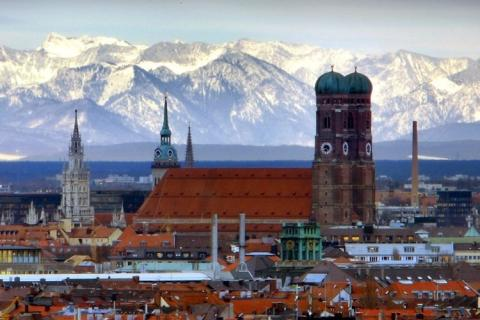
\includegraphics[width=0.31\textwidth]{./gfx/pan}
\caption{Frauenkirche med alpene i bakgrunnen}
\end{figure}




\section{Det tyske folket}
Generelt er tyskere hyggelige og imøtekommende, som nordmann er heller ikke den kulturelle forskjellen så stor. Tyskere er svært opptatt av orden og byråkrati, noe som til tider kan virke overdrevent. Den tyske humoren er noe annet hva man ser i Norge og det kan ta litt tid før man får dreisen på tankesettet. 

I de sørlige delstatene, Bayer og Baden-Württemberg, er man mer konservativ i forhold til de andre tyske delstatene. Titler og høflighet ( Sie- og du-form) er mer utbredt her, dette gjelder spesielt ovenfor proffesorer, politi og andre autoriteter.
Fyll og fest er på et roligere og et mer ''anstedig nivå'' og tyske jenter drikker langt mindre enn norske jenter. Hvordan man går kledd vil også bli, i langt større grad enn i Norge bedømmt. Det er uvanlig å se studenter i joggebukse eller tights. 
Alt dette kan virke som småpirk og noe man ikke trenger å ta hensyn til, men det blir lagt merke til. 



\section{Språket}
Tysk er generelt for nordmenn ikke spesielt vanskelig, tyskere bryr seg heller ikke så mye om man sier noe gramatisk feil så lenge det er forstålig. I starten kan det være uvant å prate tysk, men som tiden går blir man fort flinkere og alt løsner opp. Nordmenn har som regel lite problem med den tyske uttalelsen og tyskere selv skjønner ikke at de snakker med en utlending. Noen tilfeller kan det være lurt å fortelle vedkommende at man ikke er tysk, og ikke en beruset person.

Nesten alle studier i München foreleses på tysk.
Man må fremlegge dokumentasjon på at man kan nok tysk for å bli immatrikulert.
Det betyr at man må ha et DSH prøve med resultat 2 eller bedre, TestDaF med 4.4 eller bedre, Goethe med ZOP eller et diplom fra lignede institusjoner. 

En liste over noen språkkurs som godkjennes i München finner du her:\\
\url{http://www.uni-muenchen.de/studium/studium_int/studium_lmu/sprachkurse/andere_empf_deutsch/}


Her er en liste over noen godkjente språkprøver:\\
\url{http://www.uni-muenchen.de/studium/studium_int/studium_lmu/bewerbung/20_dt_nachw/}

En får tilbud om å ta en prøve rett før studiet begynner/rett før søknadsfristen. Dette kan man også ordne selv i forkant, enten i München, eller f.eks. ved Goethe-Institut i Oslo.
En skal ikke undervurdere den språkkunnskapen som trenge for enten å bestå en språkprøve eller å faktisk studere på tysk. Akademisk tysk er ikke som tysk C-språk!
  Det er ikke uvanlig å komme ned ett semester før en tenker å begynne å studere for å forberede seg og bli kjent med byen.

Dokumentasjon på påkrevd tyskkunnskap skal ved immatrikulasjonen vises. Det er helt greit å søke uten å ha beviset.

Lånekassen gir støtte til et forberedende språkkurs! \\
\url{http://www.lanekassen.no/Hovedmeny/Stipend-og-lan/Utland/Hvor-mye/Sprakstipend/}

\begin{figure}[h]
\center
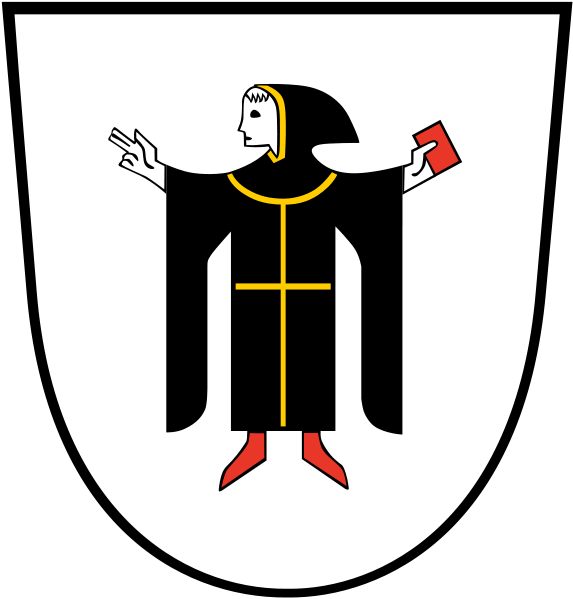
\includegraphics[width=0.15\textwidth]{./gfx/wappen}
\caption{Byvåpenet til München}
\end{figure}

\subsection{Dialekt}
Bayersk kommer i flere former og varierer i forhold til hvor personen er oppvokst. Lokalbefolkningen i München by snakker mer høytysk og er lette å forstå, derimot kan man treffe på proffesorer eller klassekamerater, som snakker bredt og nekter å endre på det. Flere tyskere som bor i Norge mener bayersk samsvarer med trøndsk. 
Men det går som regel veldig bra og er ikke et stort hinder.




\section{Ulemper ved å bo i utlandet}

Reise fra venner og familie til et sted hvor man har lite/ingen bekjennte. Feriene i Tyskland er helt anderledes enn i Norge, bortsett fra juleferien. Man har semesterferie fra tidlig feb. til sent april og sommerferie fra tidlig august til sent oktober. Dette gjør samkjøring av ferieplaner med norske venner/familie utfordrende. Det er nok enklere å studere på morsmålet, men det betyr ikke at det heller er vanskelig å studere på tysk. Det er mange som gjør det, og ende flere som har gjort det før deg. Det er veldig kult å kunne prate flytende tysk.

Ellers: Smil til livet, og livet smiler til deg.
